\documentclass{beamer}

% packages
\usepackage[utf8]{inputenc}
\usepackage[MeX]{polski}
\usepackage{hyperref}
\usepackage{graphicx}
\usepackage{pgfplots}
\usepackage{tikz, calc}
	\usetikzlibrary{arrows, shadings, shadows}
	\pgfplotsset{compat=1.8}

% theme
\usetheme{Ilmenau}
\definecolor{ios-top}{RGB}{30, 119, 239}
\definecolor{ios-bottom}{RGB}{129, 243, 254}
\definecolor{section-top}{RGB}{88, 86, 214}
\setbeamercolor{structure}{fg=ios-top}
\setbeamertemplate{blocks}[rounded][shadow=false, bg=red]
\setbeamercolor{block title}{bg=structure.fg!75!black}
\setbeamercolor{block body}{bg=structure.fg!30!white}
\setbeamertemplate{background canvas}[vertical shading][bottom=white,top=structure.fg!25]
\setbeamertemplate{sidebar canvas left}[horizontal shading][left=white!40!black,right=black]
\setbeamertemplate{itemize items}[triangle]
\setbeamercolor{section in head/foot}{fg=white,bg=structure.fg!75!black}
\setbeamercolor{alerted text}{fg=orange} 
\setbeamercolor{title in foot}{fg=white, bg=ios-top}
\setbeamertemplate{headline}
{%
  \begin{beamercolorbox}{section in head/foot}
  \vskip2pt\insertsectionnavigationhorizontal{\textwidth}{}{}\vskip2pt
  \end{beamercolorbox}
}
\setbeamertemplate{footline}
{%
  \leavevmode%
  \hbox{%
  \begin{beamercolorbox}[wd=.25\paperwidth,ht=2.25ex,dp=1ex,center]{author in head/foot}%
    \usebeamerfont{author in head/foot}\insertshortauthor
  \end{beamercolorbox}%
  \begin{beamercolorbox}[wd=.75\paperwidth,ht=2.25ex,dp=1ex,center]{title in foot}%
    \usebeamerfont{title in head/foot}\insertshorttitle\hspace*{3em}
    \insertframenumber{} / \inserttotalframenumber\hspace*{1ex}
  \end{beamercolorbox}}%
  \vskip0pt%
}
\setbeamertemplate{navigation symbols}{}

% author info 

\title[Mechanizm modelowania danych i mapowania obiektowego dla Apache Cassandry]{Praca Dyplomowa Magisterska}
\subtitle{Mechanizm modelowania danych i mapowania obiektowego dla Apache Cassandry}
\author[Jakub Turek]{Jakub Turek \\ {\small \href{mailto:J.Turek@stud.elka.pw.edu.pl}{J.Turek@stud.elka.pw.edu.pl}}}
\date{9 października 2014r.}

\begin{document}
	\titlepage

	\section{Wstęp}

	\begin{frame}
		\frametitle{Cel pracy}

		System mapowania obiektowego dla bazy Apache Cassandra:

		\begin{itemize}
			\item Zachowanie różnicy w~wydajności pomiędzy relacyjnymi bazami danych a Cassandrą.
			\item Możliwość stosowania wzorców modelowania do optymalizacji.
			\item Zachowanie zgodności z istniejącymi mechanizmami mapowania obiektowo-relacyjnego.
		\end{itemize}
	\end{frame}

	\section{ORM}
	\subsection{Kundera}

	\begin{frame}
		\frametitle{Kundera}

		\begin{block}{Kundera}
			Implementacja Java Persistence API dla baz danych NoSQL.
		\end{block}

		\vspace{10pt}

		\begin{columns}[t]
			\column{.3\textwidth}
				Wspierane silniki:

				\begin{itemize}
					\item Cassandra
					\item HBase
					\item MongoDB
					\item Redis
					\item Oracle NoSQL
					\item Neo4j
					\item Couchdb
					\item Elastic Search
				\end{itemize}

			\column{.7\textwidth}
				Porównanie czasu wstawiania rekordów:

				\vspace{20pt}

				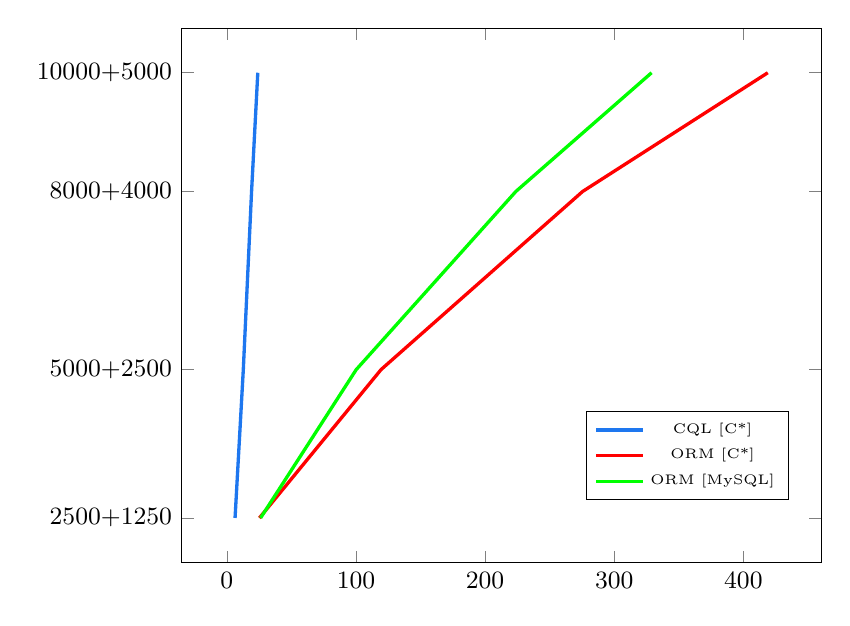
\begin{tikzpicture}
					\begin{axis}[
							width=.8\textwidth,
							scaled ticks=false, 
							tick label style={/pgf/number format/fixed},
							ytick={2500, 5000, 8000, 10000},
							yticklabels={2500+1250, 5000+2500, 8000+4000, 10000+5000},
							legend style={at={(0.95,0.2)},anchor=east,fill=none, font=\tiny},
							every axis/.append style={font=\small}
						]
						\addplot[color=ios-top, very thick] coordinates {
							(23.978, 10000)
							(19.155, 8000)
							(12.762, 5000)
							(6.366, 2500)
						};
						\addlegendentry{CQL [C*]}

						\addplot[color=red, very thick] coordinates {
							(418.915, 10000)
							(275.532, 8000)
							(119.453, 5000)
							(25.213, 2500)
						};
						\addlegendentry{ORM [C*]}

						\addplot[color=green, very thick] coordinates {
							(328.915, 10000)
							(223.823, 8000)
							(100.23, 5000)
							(26.119, 2500)
						};
						\addlegendentry{ORM [MySQL]}
					\end{axis}
				\end{tikzpicture}
		\end{columns}
	\end{frame}

  \begin{frame}
    \frametitle{This is the first slide}
    %Content goes here
  \end{frame}
  \begin{frame}
    \frametitle{This is the second slide}
    \framesubtitle{A bit more information about this}
    %More content goes here
  \end{frame}
% etc
\end{document}